\documentclass[12pt]{article}
\usepackage{amsmath, amssymb}
\usepackage{geometry}
\usepackage{graphicx}
\usepackage{parskip}

\geometry{margin=1in}

\title{ODE HW CH 8}
\author{
Greyson Knippel \\[4pt]
MATH 260-1 --- Gonzaga University \\[4pt]
Professor Jensen
}
\date{\today}

\begin{document}
\maketitle


\section*{problem 1}

predator prey system
\begin{align}
    F' &= 0.2F - 0.1FS, \label{eq:prey}\\
    S' &= -0.3S + 0.1FS, \label{eq:pred}
\end{align}
where $F(t)$ is the prey population and $S(t)$ is the predator population.

% ------------------------------------------------------------
\subsection*{(a) phase plane analysis}

all trajectories form \textbf{closed orbits} surrounding the
equilibrium point. as $F$ increases the predator population
rises; as $S$ increases the prey is driven down, as prey
declines the predators starve and decrease; and as predators decrease the
prey recovers, completing one full cycle. the populations oscillate infinitely without tending toward
either extinction or high growth.

% ------------------------------------------------------------
\subsection*{(b) solution starting at $F(0)=3$, $S(0)=2$}

the equilibrium of system~\eqref{eq:prey}--\eqref{eq:pred} is
found by setting $F'=S'=0$:
\[
    F^* = \frac{\gamma}{\delta} = \frac{0.3}{0.1} = 3,
    \qquad
    S^* = \frac{\alpha}{\beta} = \frac{0.2}{0.1} = 2.
\]
the initial condition $F(0)=3$, $S(0)=2$ fits exactly with this
equilibrium.  therefore the solution is \textbf{constant for all time}:
\[
    F(t) \equiv 3, \qquad S(t) \equiv 2, \qquad t \geq 0.
\]
both populations remain at their equilibrium values indefinitely.

\section*{problem 2}
 
\begin{align}
    x' &= 0.2x - 0.04xy, \label{eq:x}\\
    y' &= -0.1y + 0.005xy. \label{eq:y}
\end{align}
 
% ------------------------------------------------------------
\subsection*{(i) nullclines}
 
\textbf{$x$-nullclines} (set $x' = 0$):
\[
    0.2x - 0.04xy = x(0.2 - 0.04y) = 0
    \implies x = 0 \quad \text{or} \quad y = 5.
\]
 
\textbf{$y$-nullclines} (set $y' = 0$):
\[
    -0.1y + 0.005xy = y(-0.1 + 0.005x) = 0
    \implies y = 0 \quad \text{or} \quad x = 20.
\]
 
the $x$-nullclines ($x=0$ and $y=5$) and $y$-nullclines ($y=0$ and $x=20$)
are plotted in the phase plane below
 
Uncomment once nullclines.png is in the same folder as this .tex file.
\begin{figure}[h]
    \centering
    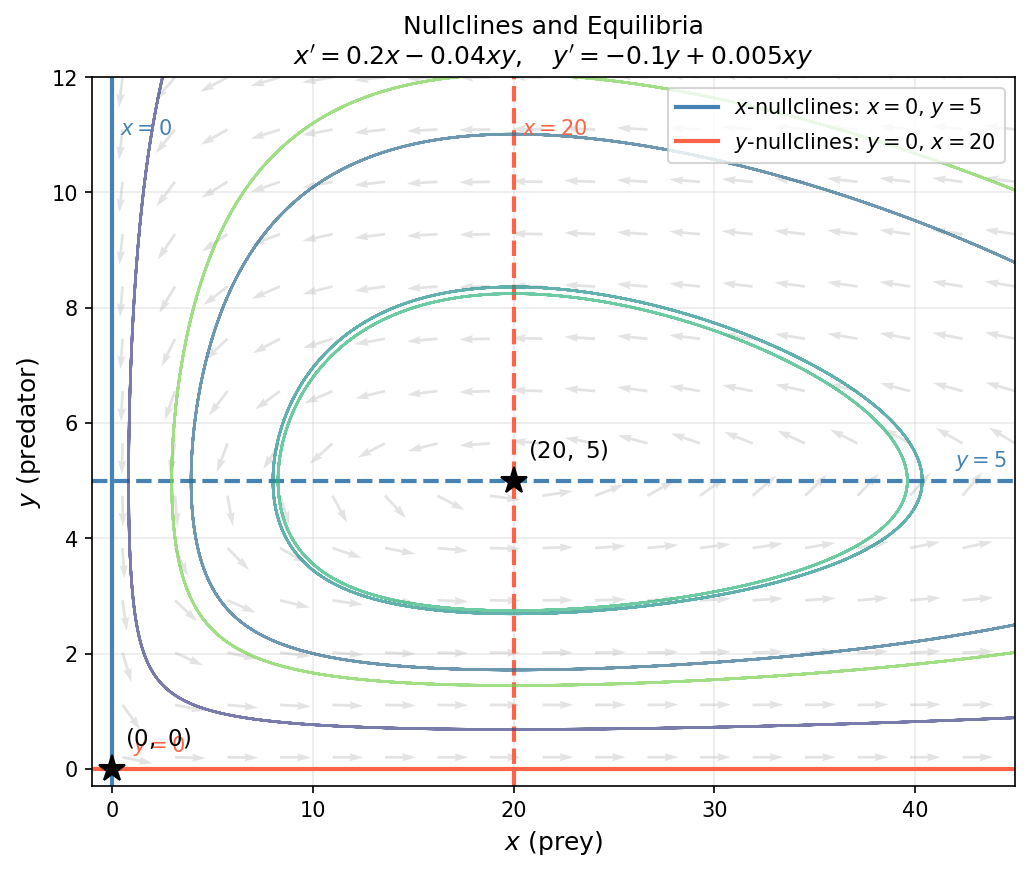
\includegraphics[width=0.72\textwidth]{nullclines.png}
    \caption{nullclines and equilibrium for
             system~\eqref{eq:x}--\eqref{eq:y}.
             blue lines are $x$-nullclines; red lines are $y$-nullclines.
             black stars mark the equilibrium points $(0,0)$ and $(20,5)$.}
    \label{fig:nullclines}
\end{figure}
 
% ------------------------------------------------------------
\subsection*{(ii) equilibrium points}
 
when an $x$-nullcline intersects a $y$-nullcline,
where $x'=0$ and $y'=0$ simultaneously.
 
\begin{center}
\renewcommand{\arraystretch}{1.3}
\begin{tabular}{ccc}
\hline
$x$-nullcline & $y$-nullcline & equilibrium \\
\hline
$x = 0$  & $y = 0$  & $(0,\,0)$ \\
$x = 0$  & $x = 20$ & $(0,\,0)$ \quad (same point) \\
$y = 5$  & $y = 0$  & $(0,\,0)$ \quad (same point) \\
$y = 5$  & $x = 20$ & $(20,\,5)$ \\
\hline
\end{tabular}
\end{center}
 
There are therefore \textbf{two distinct equilibrium points}:
\[
    (x^*, y^*) = (0,\, 0)
    \qquad \text{and} \qquad
    (x^*, y^*) = (20,\, 5).
\]
% ------------------------------------------------------------

\section*{problem 3}
 
consider the system
\begin{align}
    x_1' &= 8x_1 - 10x_2, \label{eq:sys1}\\
    x_2' &= 5x_1 - 7x_2. \label{eq:sys2}
\end{align}
 
% ------------------------------------------------------------
\subsection*{(i) matrix--vector form}
 
system~\eqref{eq:sys1}--\eqref{eq:sys2} can be written as
$\mathbf{x}' = A\mathbf{x}$, where
\[
    \mathbf{x} = \begin{pmatrix} x_1 \\ x_2 \end{pmatrix}, \qquad
    A = \begin{pmatrix} 8 & -10 \\ 5 & -7 \end{pmatrix}.
\]
which is,
\[
    \begin{pmatrix} x_1' \\ x_2' \end{pmatrix}
    =
    \begin{pmatrix} 8 & -10 \\ 5 & -7 \end{pmatrix}
    \begin{pmatrix} x_1 \\ x_2 \end{pmatrix}.
\]
 
% ------------------------------------------------------------
\subsection*{(ii) verify that $\mathbf{x}(t) = (2e^{3t},\, e^{3t})^{\mathsf{T}}$ is a solution}
 
let
\[
    \mathbf{x}(t) = \begin{pmatrix} 2e^{3t} \\ e^{3t} \end{pmatrix}.
\]
verify that $\mathbf{x}' = A\mathbf{x}$ by confirming they are equal.
 
\textbf{left side} --- differentiate $\mathbf{x}$ 
\[
    \mathbf{x}'(t)
    = \begin{pmatrix} \dfrac{d}{dt}(2e^{3t}) \\[6pt] \dfrac{d}{dt}(e^{3t}) \end{pmatrix}
    = \begin{pmatrix} 6e^{3t} \\ 3e^{3t} \end{pmatrix}.
\]
 
\textbf{right side} --- multiply $A\mathbf{x}$:
\[
    A\mathbf{x}
    = \begin{pmatrix} 8 & -10 \\ 5 & -7 \end{pmatrix}
      \begin{pmatrix} 2e^{3t} \\ e^{3t} \end{pmatrix}
    = \begin{pmatrix} 8(2e^{3t}) - 10(e^{3t}) \\ 5(2e^{3t}) - 7(e^{3t}) \end{pmatrix}
    = \begin{pmatrix} 16e^{3t} - 10e^{3t} \\ 10e^{3t} - 7e^{3t} \end{pmatrix}
    = \begin{pmatrix} 6e^{3t} \\ 3e^{3t} \end{pmatrix}.
\]
 
since $\mathbf{x}'(t) = A\mathbf{x}(t)$ for all $t$, the vector-valued
function $\mathbf{x}(t) = (2e^{3t},\, e^{3t})^{\mathsf{T}}$ is a
solution of the system. 

\end{document}